\chapVter{GoogLeNetの並列化検討}
{
\label{chap:parallel}

\section{概要}
本章ではまず,GoogLeNetの並列化検討を行う要素を明確にする.
次に並列化検討要素ごとに考察を行う.
本研究では次の3つについて並列化を検討する
\begin{itemize}
   \item Inception層 
   \item 畳み込み演算 
   \item Pooling処理 
\end{itemize}
\section{Inception層の並列化}
\label{sec:inception_para}
表\ref{table:googlenet}からもわかるようにGoogLeNetはサイズの違いはあるが,Inception層がその大半を占めている.
これがInception層に注目した理由である.
Inception層は図\ref{fig:para_inception}に示すように4つの計算に分割することができる.
\begin{figure}[h]
  \centering
  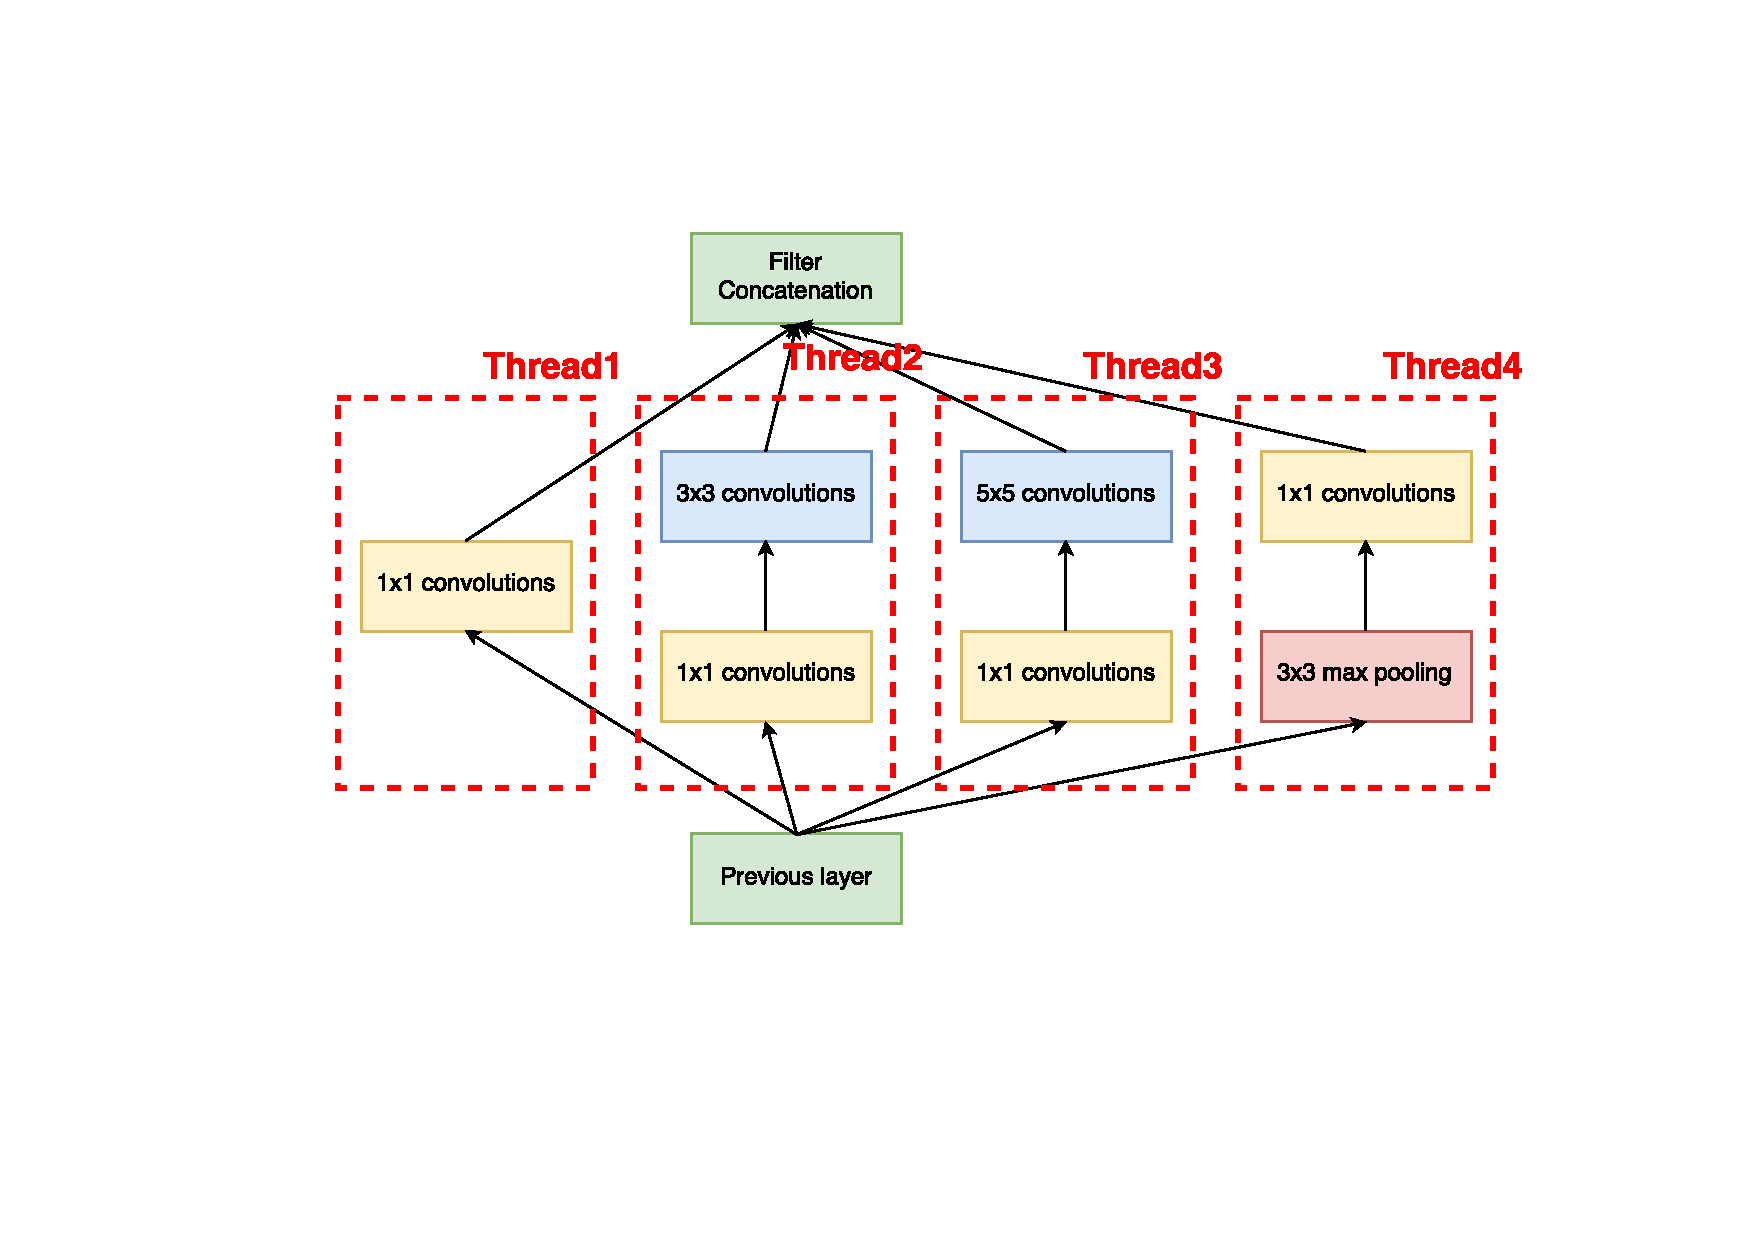
\includegraphics[width=12cm]{./chap5/fig/para_inception.pdf}
  \caption{Inception層の並列化}
  \label{fig:para_inception}
\end{figure}
便宜上図に示すようにthread1からthread4と名付けて議論する.
各スレッドには前層の出力特徴マップがそれぞれ入力特徴マップとしてブロードキャストされる.
% 各スレッドは最後にそれぞれの出力特徴マップを図\ref{fig:depth_concat}に示すように深さ方向に結合するまでの間は互いに依存せずに
% 演算を行うことができる.
% \begin{figure}[h]
%   \centering
%   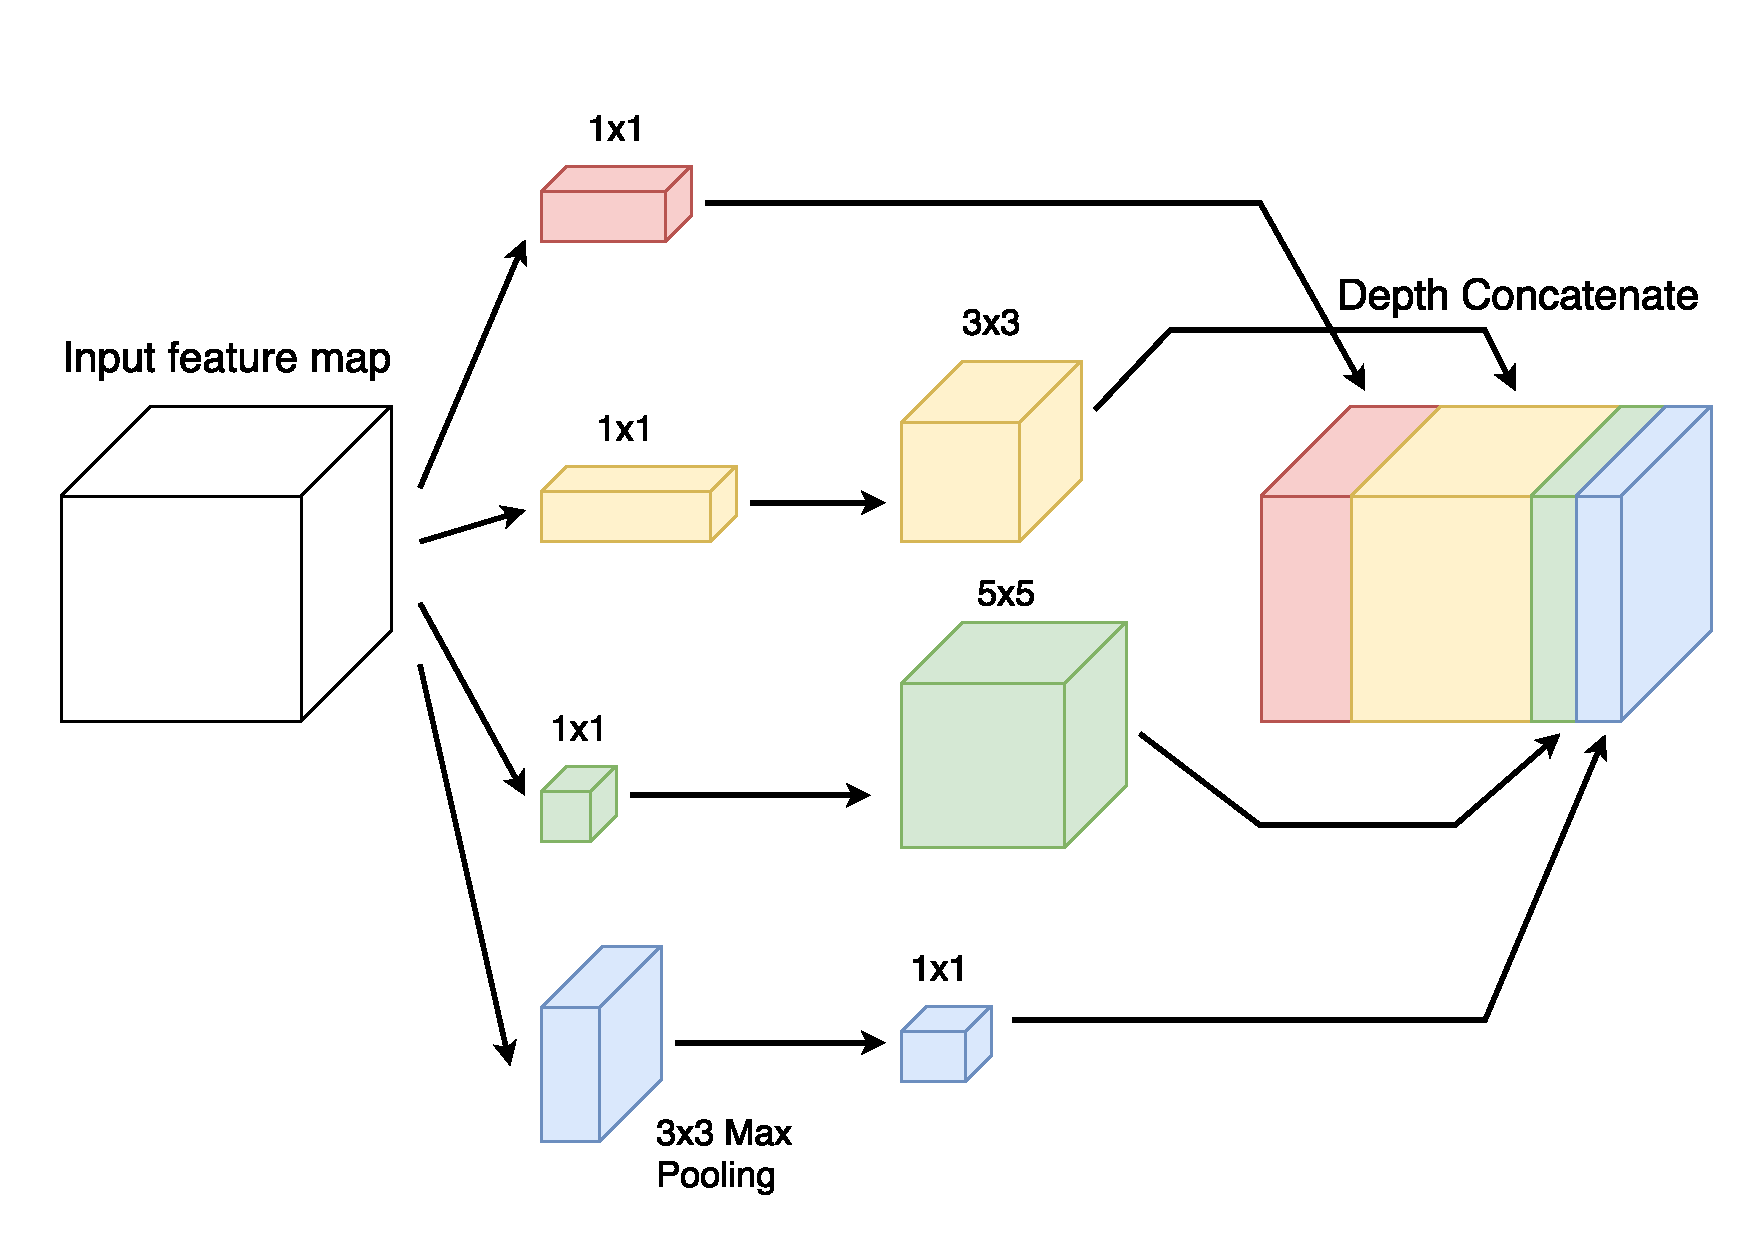
\includegraphics[width=12cm]{./chap5/fig/depthconcat.pdf}
%   \caption{}
%   \label{fig:depthconcat}
% \end{figure}
このことからInception層全体の並列化を考えると各スレッドごとに並列化することができる.
マルチFPGAに搭載する際には各スレッドごとに1枚のボードを割り当てるだけでなく,計算処理の重たいスレッドに関しては,
スレッド内の畳込み演算部などを並列に処理することができるので,あるスレッド内の処理も複数FPGAボードに割り当てることが可能である.

\section{畳み込み演算の並列化}
\label{sec:conv_para}
畳み込み演算の並列化を検討する.
CNNはその名の通り畳み込み演算が主演算となるのでこの並列化は様々な研究で検討される.
畳み込み演算はその演算の性質上,とくにデータ並列度が高い.
本研究では重みフィルタパラメータを各FPGAボードのローカルメモリ(BRAM)に保存し,外部からの入力特徴マップとの演算を行い,出力特徴マップを
求めるという設計を行う.これはあるFPGAがネットワークの特定の層のある箇所のみの演算を行い次々とFPGAボードを伝搬させていくという設計方針を満たす
ためである.次々と入力値をFPGAが受け取りストリーム処理を行うことを想定している.
畳み込み演算の並列化には次のようなものが考えられる.
\begin{itemize}
    \item 出力値分割
    \item 入力値分割
\end{itemize}
\subsection{出力値分割}
\label{subsec:para_output}
出力特徴マップを分割することを考える.出力特徴マップ同士には依存性がないが,次層での入力値となることを考えると,
すべての特徴出力マップが揃うのを待つ必要がある.
この並列化の様子を図\ref{fig:}に示す.
\begin{figure}[h]
    \centering
    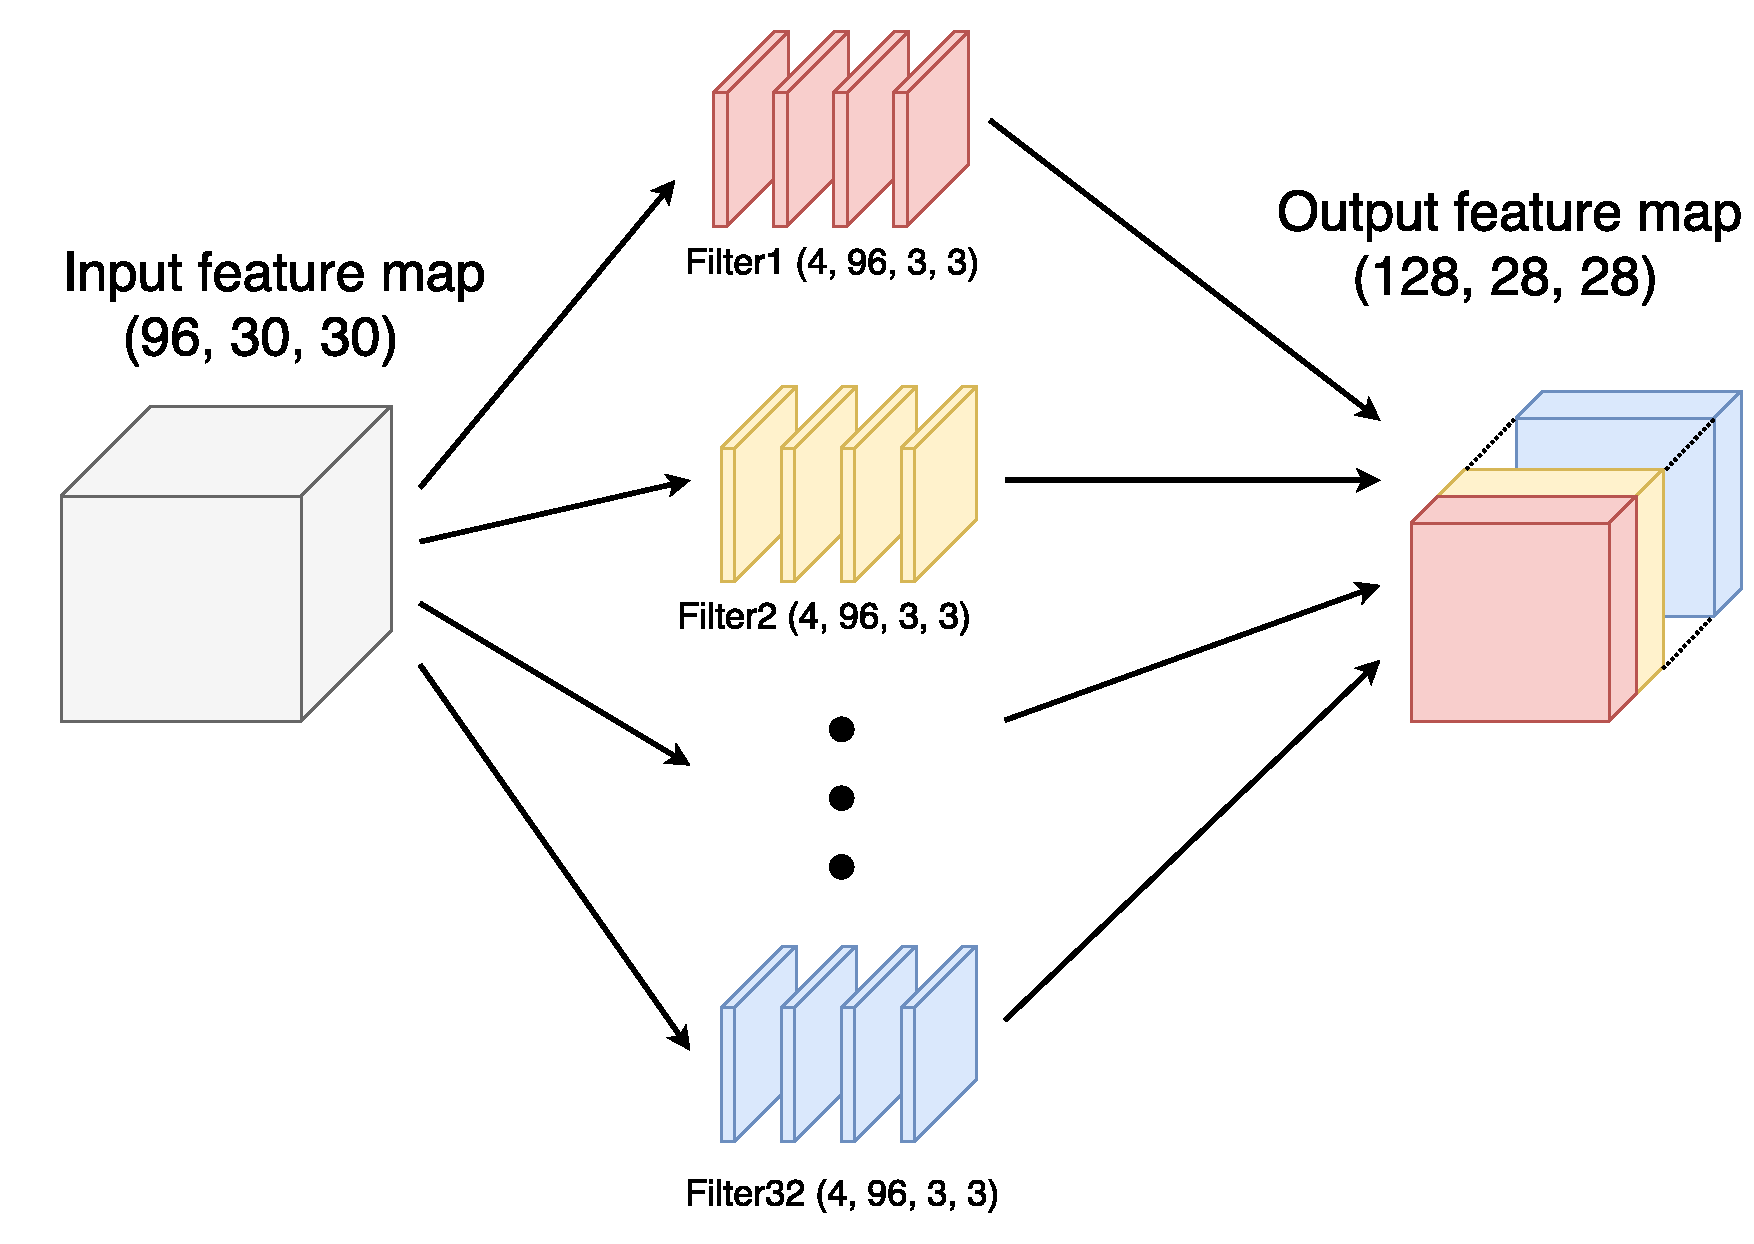
\includegraphics[width=12cm]{./chap5/fig/conv_para_output.pdf}
    \caption{出力値分割}
    \label{fig:conv_para_output}
\end{figure}
図中ではInception3a層のthread2の3$\times$3畳み込み演算の入出力サイズを用いている.
入力サイズ(96,30,30) に対して重みフィルタサイズ(128, 96, 3, 3)の重みとの演算を行い,出力サイズ(128,28,28)に対して,32並列化を実行している.
並列化された各ノードは入力サイズ(96,30,30)を受け取り出力サイズ(4,28,28)を出力する.
こうすることで逐次的に処理するときと比較して理論的には32倍の速度性能を達成することができる.
しかし演算の最後に並列演算したそれぞれの出力特徴マップをDepthConcat層の処理のように深さ方向での結合をしなければならない.
\subsection{入力値分割}
\label{subsec:para_input}
入力値について並列化することも考えられる.入力特徴マップのサイズが大きいものについて
分割して処理することでスループットの向上の可能性がある.
この並列化の様子を図\ref{fig:para_input}に示す.
\begin{figure}[h]
    \centering
    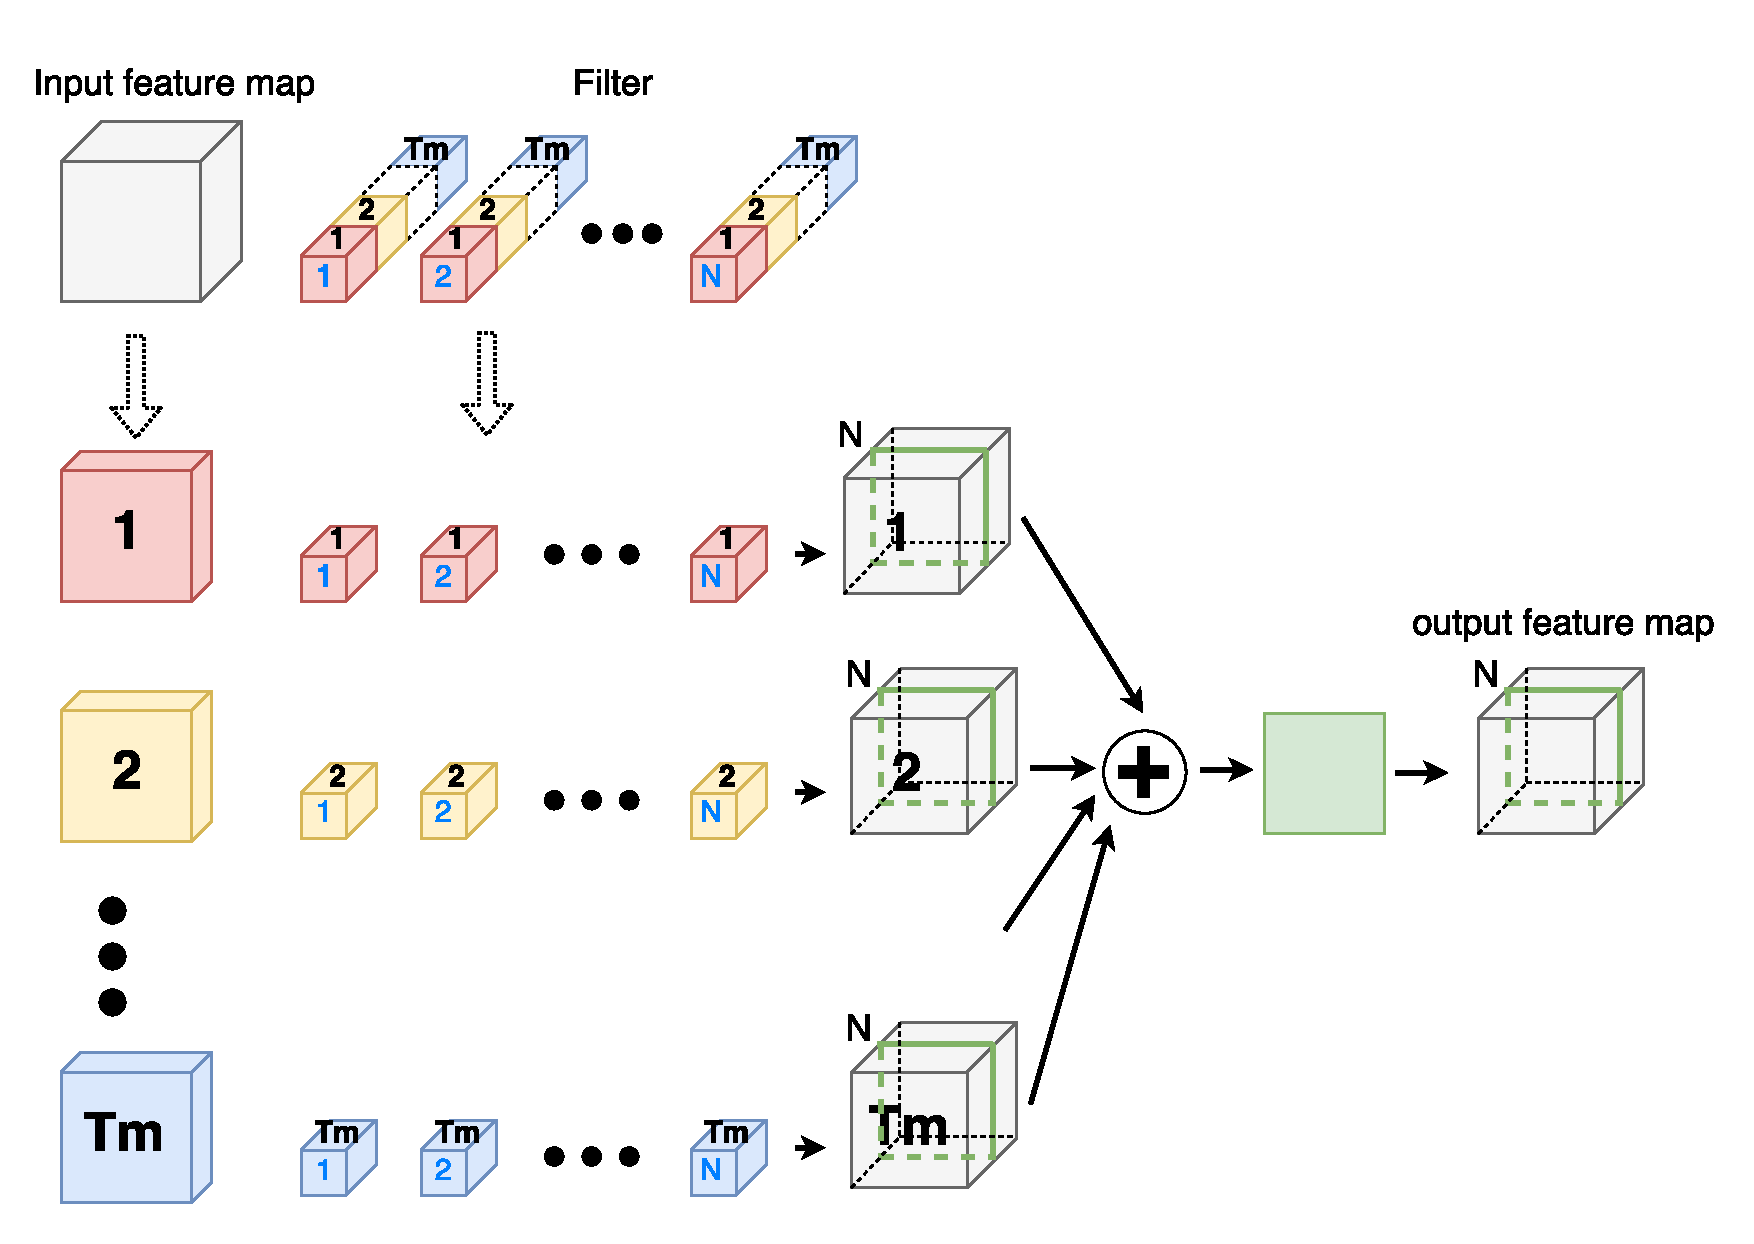
\includegraphics[width=12cm]{./chap5/fig/conv_para_input.pdf}
    \caption{入力値分割}
    \label{fig:conv_para_input}
\end{figure}
ここでも同じくInception3a層のthread2の3$\times$3畳み込み演算の入出力サイズを用いて説明する.
16個に入力特徴マップを分割するとそれぞれ(6,30,30)の入力サイズとなる.これに対し128個の(96,3,3)のサイズも16個に分割し(6,3,3)のサイズにする.
分割された入力特徴マップは対応する128個の分割された重みフィルタと畳込み演算を行い(128,28,28)の中間特徴マップを得る.
この16個の中間特徴マップのそれぞれの深さd$(1 \leq d \leq 128)$の二次元特徴マップの総和をとることで最終的な出力特徴マップの深さdの二次元特徴マップが得られる.
この操作を各dに対して行うことで最終的な出力特徴マップを得ることができる.
分割された入力特徴マップと重みフィルタはそれぞれ並列に演算が可能である.

}